\chapter{Giovedì 14/05/2020}
\section{Locking a due fasi stretto (o rigoroso)}
Ci siamo lasciati con due anomalie ancora da risolvere: le letture sporche e le \emph{deadlock}. Per risolvere il primo problema si ricorre a un locking \emph{a due fasi stretto}. Si impone un'ulteriore condizione:
\begin{itemize}
	\item I lock possono essere rilasciati \underline{solo} dopo aver fatto commit.
\end{itemize}
In questo modo gli stati intermedi non saranno visibili finchè non si avrà il commit! A quel punto siamo certi che le transazioni non saranno annullate.
\paragraph{Confronto tra schedule no 2PL (a destra) e schedule con 2PL stretto (a sinistra)}
\begin{center}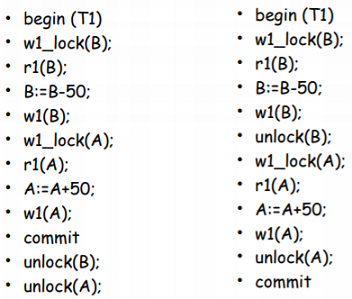
\includegraphics{images/169.PNG}\end{center}
\section{Alternativa: controllo di concorrenza basato su timestamp}
Questa è una tecnica alternativa al 2PL.  Ogni transazione è identificata in modo univoco attraverso un \emph{timestamp}. Ci baseremo sull'ordine con cui sono state attivate le transazioni
\paragraph{Accettazione degli schedule} Lo schedule deve essere equivalente allo schedule che riflette l'ordinamento delle transazioni (indotto dai timestamp).
\paragraph{Esempio} Immaginiamo di avere le transazioni 
\[T_1,T_2,T_3\]
attivate nell'ordine indicato (immaginiamo che gli indici identificativi siano i timestamp). Gli unici ordinamenti seriali accettabili sono quelli compatibili con l'ordine seriale delle transazioni. Segue che uno schedule equivalente a questo
\[T_2,T_1,T_3\]
non va bene.
\paragraph{Dettagli}
\begin{itemize}
	\item Tutti gli oggetti coinvolti dallo scheduler presentano due contatori: 
	\begin{itemize}
		\item uno per le letture $RTM(x)$: consiste nel timestamp \underline{massimo} tra quelli associati alle transazioni che hanno letto l'oggetto $x$
		\item uno per le scritture $WTM(x)$: consiste nel timestamp dell'ultima transazione che ha scritto sull'oggetto $x$
	\end{itemize}
	\item Lo scheduler riceve richieste di letture e scritture (assieme al timestamp della transazione):
	\begin{itemize}
		\item lettura \emph{read(x,ts)}:
		\begin{itemize}
			\item se $\boxed{ts < WTM(x)}$ la richiesta è respinta e la transazione abortita
			\item negli altri casi accolgo la richiesta ponendo $\boxed{RTM(x) = \max(RTM(x),ts)}$
		\end{itemize}
		\item scrittura \emph{write(x,ts)}:
		\begin{itemize}
			\item Se $\boxed{ts < RTM(x)}$ \underline{o} $\boxed{ts < WTM(x)}$ la richiesta è respinta e la transazione abortita
			\item negli altri casi la richiesta viene accolta ponendo $\boxed{WTM(x) = ts}$
		\end{itemize}
	\end{itemize}
\end{itemize}
\paragraph{Esempio} 
\begin{center}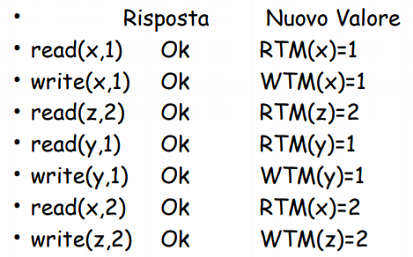
\includegraphics{images/170.PNG}\end{center}
\pagebreak


\subsection{2PL e TS} Gli schedule TS sono automaticamente CSR: corrispondono ad una esecuzione seriale (quella in cui le transazioni sono eseguite nell'ordine in cui sono iniziate). Tuttavia 2PL e TS sono incomparabili!
\begin{center}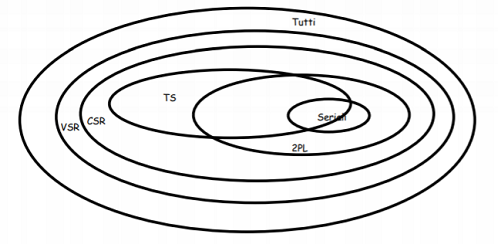
\includegraphics{images/171.PNG}\end{center}
\paragraph{Attenzione} L'ordine seriale delle transazioni è fissato prima che le operazioni vengano richieste. Altri ordinamenti non sono accettati.
\subparagraph{Situazione} Quando $T1$ comincia prima di $T2$ potrebbe essere abilitato uno schedule 2PL o CSR equivalente ad uno seriale $T2\;T1$. Col TS ciò non è possibile, al limite uccido la $T1$ per poi farla ripartire dopo $T2$.
\paragraph{Quindi}
\begin{itemize}
	\item In $2PL$ la transazioni sono poste in attesa quando il lock non può essere acquisito. In $TS$ vengono uccise e rilanciate.
	\item il $2PL$ conviene maggiormente poichè la ripartenze in $TS$ sono più costose delle attese.
	\item Tuttavia il $2PL$ può causare \emph{deadlock}. Mediamente si uccide una transazione ogni due conflitti, ma la probabilità di insorgenza di deadlock è molto minore della probabilità di un conflitto. Segue che il $2PL$ rimane la scelta migliore.
\end{itemize}
\subsection{Risoluzione dello stallo}
Vogliamo mantenere il $2PL$ e risolvere il problema del \emph{deadlock}. La maggior parte dei sistemi in commercio adotta la metodologia del \emph{timeout}:
\begin{itemize}
	\item Le transazioni rimangono in attesa di una rirsorsa per un tempo prefissato. 
	\item Se, trascorso tale tempo, la risorsa non è stata ancora concessa, alla richiesta di lock viene data risposta negativa. 
	\item In tal modo una transazione in potenziale stato di deadlock viene tolta dallo stato di attesa e di norma abortita. 
\end{itemize}
Un valore troppo elevato tende a risolvere tardi i blocchi critici. Un valore troppo basso rischia di interpretare come blocchi anche situazioni in cui una transazione sta attendendo la disponibilità di una risorsa destinata a liberarsi, uccidendo la transazione e sprecando il lavoro già svolto.
\paragraph{Come scelgo la transazione da uccidere} 
\begin{itemize}
	\item Politiche interrompenti:
	\begin{itemize}
		\item Un conflitto può essere risolto uccidendo la transazione che possiede la risorsa (in tal modo questa rilascia la risorsa). 
		\item Un criterio aggiuntivo potrebbe essere uccidere le transazioni che hanno svolto minore lavoro.
	\end{itemize}
	\item Politiche non interrompenti: una transazione può essere uccisa solo nel momento in cui effettua una nuova richiesta.
\end{itemize}
\paragraph{Conseguenza del criterio aggiuntivo} Il problema fondamentale è che una transazione, all'inizio, accede ad un oggetto richiesto da altre transazioni. Risulta presente un conflitto e segue che questa sarà ripetutamente uccisa. Non ho un deadlock, ma \emph{starvation}.
\subparagraph{Soluzione?} Mantenere invariato il timestamp delle transazioni abortite, dando in questo modo priorità alle transazioni più anziane.
\subsubsection{Esempi}
Abbiamo la seguente transazione
\[S: r1(y)w3(z)r1(z)r2(z)w3(x)w1(x)w2(x)r3(y)\]
Vogliamo mostrare l'esecuzione delle operazioni in $S$ quando
\begin{itemize}
	\item è applicato il two phase locking stretto
	\item è applicato il protocollo basato su timestamp
\end{itemize}
\begin{multicols}{2}
	\paragraph{2PL}
	\begin{center}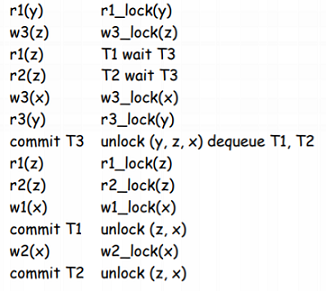
\includegraphics{images/172.PNG}\end{center}
	\paragraph{TS}
	\begin{center}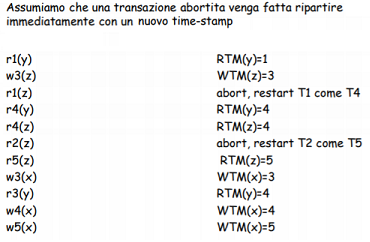
\includegraphics{images/173.PNG}\end{center}
\end{multicols}
\pagebreak

\section{Dettagli riguardanti SQL}
Le transazioni sono partizionate in \emph{read-only} e transazioni \emph{read-write} (queste di default). Le prime non possono modificare nè il contenuto nè lo schema della base di dati e si basano esclusivamente su \emph{lock condivisi}.
\paragraph{read-only} Di queste possiamo scegliere un certo livello di isolamento. Ciò significa accettare delle anomalie.
\begin{itemize}
	\item \textbf{read uncommitted}: possibili letture sporche, letture inconsistenti, aggiornamenti fantasma e inserimenti fantasma (niente lock in lettura, assenza di rispetto per i lock altrui)
	\item \textbf{read committed}: evito letture sporche ma permetto letture inconsistenti, aggiornamenti fantasma e inserimenti fantasma (lock in lettura, senza $2PL$)
	\item \textbf{repeatable read}: evito tutte le anomalie tranne gli inserimenti fantasma ($2PL$ anche in lettura)
	\item \textbf{serializable}: evito tutte le anomalie ($2PL$)
\end{itemize}
La perdita di aggiornamento è evitata in ogni caso.
\paragraph{read-write} Il $2PL$ stretto è sempre utilizzato nelle scritture. Quindi si evitano tutte le anomalie (in particolare la perdita di aggiornamento)
\textit{\paragraph{Ricapitoliamo}
	\begin{itemize}
		\item \textbf{Perdita di aggiornamento (W-W)}: Abbiamo due transazioni che effettuano operazioni di scrittura su un oggetto. Le operazioni si basano su una precedente lettura. Il problema è che una delle letture non legge il dato aggiornato: segue che una delle due modifiche risulta persa!
		\item \textbf{Lettura sporca (R-W o W-W con abort)}: ho una transazione che legge e scrive e una che legge. La prima transazione abortisce, ma la seconda nel frattempo ha letto il valore di $x$ modificato.
		\item \textbf{Letture inconsistenti (R-W)}: ho una transazione che svolge due operazioni di lettura e una che svolge un'operazione di lettura seguita da una di scrittura. In uno schedule serializzabile non è possibile che le due operazioni di lettura restituiscano valori diversi!
		\item \textbf{Aggiornamento fantasma (R-W)}: Abbiamo una transazione che legge dei valori aggiornati da un'altra transazione. L'interleaving potrebbe portare alla violazione di vincoli precedentemente imposti.
		\item \textbf{Inserimento fantasma (R-W)}: una transazione potrebbe effettuare una lettura di una serie di valori e successivamente usarli per calcolare un risultato. Tra la prima e la seconda cosa si ha l'inserimento, da parte di una seconda transazione, di un nuovo valore: questo sarà ignorato.
\end{itemize}}